\documentclass{article}

\usepackage{Vor2018skil}

\title{Tölvunarfræði 2, \semester \\ Skilaverkefni 7}
\author{}

\begin{document}
\maketitle
\hypersetup{pdftitle={Tölvunarfræði 2 - Skilaverkefni 7}}

Skila skal þessum verkefnum á \href{https://gradescope.com/courses/14122}{Gradescope}.

Þegar forriti er skilað inn til yfirferðar er mikilvægt að láta \textbf{niðurstöðurnar fylgja}. Öllum forritskóða skal skila framsettum með jafnbilaletri. Hann þarf að vera afritanlegur úr .pdf skjalinu. Vönduð framsetning og læsilegur kóði er hluti af verkefninu.

\question

Klasinn \href{https://algs4.cs.princeton.edu/code/edu/princeton/cs/algs4/BST.java.html}{BST.java} táknar nafnatöflu með samanburðarhæfum lyklum. Hann inniheldur aðferðirnar \texttt{min} og \texttt{max} til að finna útgildi töflunnar.

Þessar aðferðir eru útfærðar með endurkvæmni. Það gerir kóðann knappan og fágaðan\footnote{Skv. gildismati kennarans.}, en getur valdið vandræðum verði tvíleitartréð sem liggur að baki töflunni mjög langt frá því að vera í jafnvægi.

Breytið útfærslunum á (public) \texttt{min()} og \texttt{max()} aðferðunum svo að þær noti ítrun í stað endurkvæmni. Skilið breyttu aðferðunum ásamt dæmi um keyrslu á gefnum \href{https://github.com/Ernir/kennsluefni/tree/master/T2/Code/w8/stringsearchtree.java}{prufuklasa}.

\paragraph{Ábending 1:} Afritið \texttt{BST.java} í vinnumöppuna ykkar og breytið því eintaki. Prufuklasinn keyrir ekki án þess.

\paragraph{Ábending 2:} Mjög gagnlegt er að nota debugger til að skoða uppbyggingu breytunnar \texttt{bst} rétt áður en keyrslu prufuforritsins lýkur til að átta sig á uppbyggingu tvíleitartrésins.

\question

Skrifið forrit sem framkvæmir endurteknar mælingar á \href{https://algs4.cs.princeton.edu/code/edu/princeton/cs/algs4/BinarySearchST.java.html}{BinarySearchST}.

Mælið keyrslutíma uppflettingar á slembivöldum lykli í nafnatöflum sem innihalda frá 50000 upp í 5000000 aðskilda heiltölulykla. 

Prófið stærðirnar $50000, 100000, 150000, \ldots , 5000000$. Til að fá betra mat skuluð þið framkvæma röðunina 20000 sinnum fyrir hverja stærð á fylki og reikna meðalkeyrslutímann. Veljið nýjan lykil í hverri einustu keyrslu (20000 mismunandi lyklar fyrir hverja stærð verða prófaðir).

Teiknið að lokum niðurstöðurnar upp sem safn af punktum, með fjölda lykla á lárétta ásnum og meðalkeyrslutímann fyrir töflunni af þeirri stærð á lóðrétta ásnum. Niðurstaðan ætti að vera svipuð og á mynd \ref{mynd:1}.

\newpage

Sérstök beinagrind er ekki gefin, en grunnstærðirnar eru eftirfarandi:

\begin{minted}{java}
int maxArraySize = 5000000;  // Mesta stærð á fylki sem við ætlum að tímamæla
int stride =       50000;    // Bil á milli stærða
int numTrials =    20000;    // Fjöldi mælinga fyrir hverja stærð fylkis
\end{minted}

Hugmyndir (og beinagrindin) úr skilaverkefni 5 geta verið gagnlegar.

\begin{figure}[h]
	\caption{Keyrslutími helmingunarleitar eftir inntaksstærð. Ef vel er gáð má sjá logra.}
	\label{mynd:1}
	\begin{center}
		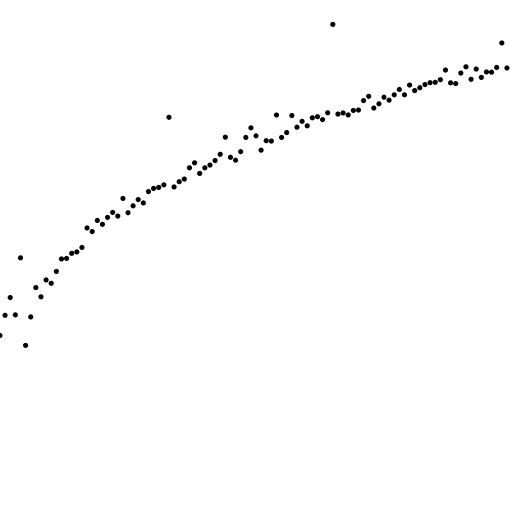
\includegraphics[width=0.5\textwidth]{binary-search-times}
	\end{center}
\end{figure}

\paragraph{Ábending 1} Valkvæmt er að festa grunntölu slembitölugjafans.
\paragraph{Ábending 2} Forritið tók tæplega 20 sekúndur í keyrslu á tölvu kennarans. Gagnlegt er að nota aðrar tölur (t.d. lægra \texttt{maxArraySize} og hærra \texttt{stride}) meðan á forritun stendur.
\paragraph{Ábending 3} Grunnstærðirnar eru ekki heilagar. Vera má að þessar tölur gefi slæma (eða enga) mynd á ykkar tölvu. Takið fram ef þið neyðist til að breyta þeim.

\question

Í \texttt{algs4.jar} sjáum við tvíleitartré til að útfæra nafnatöflu eins og \href{https://algs4.cs.princeton.edu/code/edu/princeton/cs/algs4/BST.java.html}{BST.java}. Þar eru lyklar \eng{keys} og gildi \eng{values} aðskilin fyrirbrigði. Þetta er gagnlegt til að geta flett upp gildum eftir lyklum.

En ef þarfir okkar eru minni, t.d. ef það eina sem við þurfum að gera er að geyma gögn og athuga síðar hvort við höfum skráð þau áður getum við notað örlítið einfaldari útfærslu á tvíleitartré. Þetta krefst þess að gögnin sem geymd eru séu samanburðarhæf. Strengir (hér \texttt{std::string}) í C++ eru dæmi um samanburðarhæf gögn. 

Skrifið tvíleitartré í C++ sem styður aðgerðirnar \texttt{put} og \texttt{contains} í samræmi við lýsingu í \href{https://github.com/Ernir/kennsluefni/tree/master/T2/Code/w8/stringsearchtree.cpp}{beinagrind}. Útfærið einnig útskrift trésins á staðalstraum (í réttri röð).

Ekki breyta \texttt{main} fallinu eða haus fallanna og aðferðanna sem á að útfæra. 

\newpage
Dæmi um útskrift (lína 2 er breytileg):
\begin{verbatim}
$ ./stringsearchtree
Setjum ávexti í tréð í eftirfarandi röð:
Mandarína Greip Sítróna Stjörnuávöxtur Ananas Mangó Epli Banani Melóna Súraldin

Allir ávextirnir lentu í trénu.
Engin ferskja er í trénu, sem er eðlilegt.

Skrifum út ávextina í trénu í réttri röð:
Ananas Banani Epli Greip Mandarína Mangó Melóna Stjörnuávöxtur Sítróna Súraldin
\end{verbatim}

\vfill

\includegraphics[width=0.5\linewidth]{hi-von-logo}
\end{document}